%\documentclass[serif, mathserif, professionalfont]{beamer}
\documentclass[14pt,aspectratio=1610]{beamer}
\usetheme{Boadilla}
\usefonttheme{professionalfonts}

%\usecolortheme{dove}
%\usenavigationsymbolstemplate{}
%\usetheme[
%        menuwidth={0.3\paperwidth}
%        ]{amznbln}

\setbeamercovered{transparent=20}

\setlength{\parskip}{0.05cm}

\setlength{\parskip}{1em}

\usepackage[makeroom]{cancel}
\usepackage{verbatim}

\usepackage{algorithmic,multirow,colortbl}
\usepackage{animate}
\usepackage{tikz}
\usepackage{natbib}
\newcommand{\tikzmark}[1]{\tikz[overlay, remember picture] \coordinate (#1);}
\usepackage{appendixnumberbeamer}

%\usetheme[
%        menuwidth={0.3\paperwidth}
 %       ]{amznbln}

%\setbeamercolor{framesubtitle}{fg=red}
%\addtobeamertemplate{frametitle}{}{%
%  \ifx\insertframesubtitle\@empty\else%
%  \usebeamerfont{framesubtitle}%
%  \usebeamercolor[fg]{framesubtitle}%
%  \insertframesubtitle%
%  \fi%
%}

\setbeamercovered{transparent=20}
% This file defines macros, notation is defined in notationDef.tex
\usepackage{color}
\usepackage{verbatim}

\global\long\def\neil#1{\textbf{\color{red}#1}}
%\global\long\def\todo#1{\textbf{TODO: #1}}
\global\long\def\instructions#1{\textbf{INSTRUCTIONS: #1}}

\definecolor{brown}{rgb}{0.9,0.59,0.078}
\definecolor{ironsulf}{rgb}{0,0.7,.5}
\definecolor{lightpurple}{rgb}{0.156,0,0.245}

\newenvironment{matlab}{\comment}{\endcomment}
\newenvironment{octave}{\comment}{\endcomment}
\newenvironment{matlabv}{\verbatim}{\endverbatim}
\newenvironment{octavev}{\verbatim}{\endverbatim}

\ifdefined\blackBackground
\definecolor{colorOne}{rgb}{0, 1, 1}
\definecolor{colorTwo}{rgb}{1, 0, 1}
\definecolor{colorThree}{rgb}{1, 1, 0}
\definecolor{colorTwoThree}{rgb}{1, 0, 0}
\definecolor{colorOneThree}{rgb}{0, 1, 0}
\definecolor{colorOneTwo}{rgb}{0, 0, 1}
\else
\definecolor{colorOne}{rgb}{1, 0, 0}
\definecolor{colorTwo}{rgb}{0, 1, 0}
\definecolor{colorThree}{rgb}{0, 0, 1}
\definecolor{colorTwoThree}{rgb}{0, 1, 1}
\definecolor{colorOneThree}{rgb}{1, 0, 1}
\definecolor{colorOneTwo}{rgb}{1, 1, 0}
\fi

\ifdefined\blackBackground
\global\long\def\redColor{cyan}
\global\long\def\greenColor{magenta}
\global\long\def\blueColor{yellow}
\global\long\def\magentaColor{green}
\global\long\def\blackColor{white}
\global\long\def\whiteColor{black}
\else
\global\long\def\redColor{red}
\global\long\def\greenColor{green}
\global\long\def\blueColor{blue}
\global\long\def\magentaColor{magenta}
\global\long\def\blackColor{black}
\global\long\def\whiteColor{white}
\fi

\global\long\def\det#1{\left|#1\right|}
\global\long\def\erf{\text{erf}}
\global\long\def\refeq#1{(\ref{#1})}
\global\long\def\refsec#1{Section \ref{#1}}
\global\long\def\refsecs#1#2{Sections \ref{#1}--\ref{#2}}
\global\long\def\reftwosec#1#2{Sections \ref{#1} and \ref{#2}}
\global\long\def\Refsec#1{Section \ref{#1}}

% Try and avoid these macros for notation, they are definitions of convenience.
\global\long\def\bfdelta{\boldsymbol{\delta}}
\global\long\def\bfDelta{\boldsymbol{\Delta}}
\global\long\def\bfbeta{\boldsymbol{\beta}}
\global\long\def\bfgamma{\boldsymbol{\gamma}}
\global\long\def\bfmu{\boldsymbol{\mu}}
\global\long\def\bfnu{\boldsymbol{\nu}}
\global\long\def\bfalpha{\boldsymbol{\alpha}}
\global\long\def\bfepsilon{\boldsymbol{\epsilon}}
\global\long\def\bfSigma{\boldsymbol{\Sigma}}
\global\long\def\bftau{\boldsymbol{\tau}}
\global\long\def\bflambda{\boldsymbol{\lambda}}
\global\long\def\bfLambda{\boldsymbol{\Lambda}}
\global\long\def\bfpsi{\boldsymbol{\psi}}
\global\long\def\bfxi{\boldsymbol{\xi}}
\global\long\def\bfpi{\bm{\pi}}
\global\long\def\bfPsi{\boldsymbol{\Psi}}
\global\long\def\bfphi{\boldsymbol{\phi}}
\global\long\def\bfPhi{\boldsymbol{\Phi}}
\global\long\def\bfrho{\boldsymbol{\rho}}
\global\long\def\bftheta{\boldsymbol{\theta}}
\global\long\def\bfTheta{\boldsymbol{\Theta}}
\global\long\def\bfomega{\boldsymbol{\omega}}


\global\long\def\Bmath#1{\boldsymbol{#1}}


% Avoid these macros for notation, they are definitions of convenience.
\global\long\def\bfa{\mathbf{a}}
\global\long\def\bfb{\mathbf{b}}
\global\long\def\bfc{\mathbf{c}}
\global\long\def\bfd{\mathbf{d}}
\global\long\def\bfe{\mathbf{e}}
\global\long\def\bff{\mathbf{f}}
\global\long\def\bfg{\mathbf{g}}
\global\long\def\bfh{\mathbf{h}}
\global\long\def\bfk{\mathbf{k}}
\global\long\def\bfl{\mathbf{l}}
\global\long\def\bfm{\mathbf{m}}
\global\long\def\bfn{\mathbf{n}}
\global\long\def\bfo{\mathbf{o}}
\global\long\def\bfp{\mathbf{p}}
\global\long\def\bfq{\mathbf{q}}
\global\long\def\bfr{\mathbf{r}}
\global\long\def\bfs{\mathbf{s}}
\global\long\def\bft{\mathbf{t}}
\global\long\def\bfu{\mathbf{u}}
\global\long\def\bfv{\mathbf{v}}
\global\long\def\bfw{\mathbf{w}}
\global\long\def\bfx{\mathbf{x}}
\global\long\def\bfy{\mathbf{y}}
\global\long\def\bfz{\mathbf{z}}

\newcommand{\dif}[1]{\text{d}#1}
\global\long\def\cov{\text{cov}}


\global\long\def\bfzero{\mathbf{0}}
\global\long\def\bfone{\mathbf{1}}


\global\long\def\bfA{\mathbf{A}}
\global\long\def\bfB{\mathbf{B}}
\global\long\def\bfC{\mathbf{C}}
\global\long\def\bfD{\mathbf{D}}
\global\long\def\bfE{\mathbf{E}}
\global\long\def\bfG{\mathbf{G}}
\global\long\def\bfH{\mathbf{H}}
\global\long\def\bfI{\mathbf{I}}
\global\long\def\eye{\mathbf{I}}
\global\long\def\bfK{\mathbf{K}}
\global\long\def\bfL{\mathbf{L}}
\global\long\def\bfM{\mathbf{M}}
\global\long\def\bfO{\mathbf{O}}
\global\long\def\bfP{\mathbf{P}}
\global\long\def\bfQ{\mathbf{Q}}
\global\long\def\bfR{\mathbf{R}}
\global\long\def\bfS{\mathbf{S}}
\global\long\def\bfT{\mathbf{T}}
\global\long\def\bfU{\mathbf{U}}
\global\long\def\bfV{\mathbf{V}}
\global\long\def\bfW{\mathbf{W}}
\global\long\def\bfX{\mathbf{X}}
\global\long\def\bfY{\mathbf{Y}}
\global\long\def\bfZ{\mathbf{Z}}
\global\long\def\llangle{{\langle\vspace{-2mm} \langle}}
\global\long\def\rrangle{{\rangle\vspace{-2mm} \rangle}}
\global\long\def\la{\leftarrow}


\global\long\def\tf{\tilde{f}}
\global\long\def\tg{\tilde{g}}
\global\long\def\tX{\tilde{X}}
\global\long\def\tY{\tilde{Y}}
\global\long\def\tZ{\tilde{Z}}


\global\long\def\bbE{\mathbb{E}}
\global\long\def\bbR{\mathbb{R}}
\global\long\def\bbP{\mathbb{P}}
\global\long\def\bbT{\mathbb{T}}
\global\long\def\bbZ{\mathbb{Z}}


\global\long\def\ois{2 \pi i s}
\global\long\def\oik{2 \pi i k}
\global\long\def\oin{2 \pi i n}
\global\long\def\oim{2 \pi i m}


\global\long\def\T{{\top}}
\global\long\def\Tr{\mbox{Tr}}
\global\long\def\trace#1{\text{tr}\left(#1\right)}
%\global\long\def\diff#1{{\, d#1}}
\global\long\def\diff#1#2{\frac{\text{d}#1}{\text{d}#2}}
\global\long\def\vgraph#1{ \newpage\begin{center} \end{center}{center}{center}{center}{center}{center}{center}{center}{center}{center}{center}{center}{center}{center}{center}{center}{center} {\large{\bf #1}} {center} \vspace{2mm} }
\global\long\def\high#1{\textcolor{blue}{\emph{#1}}}
\global\long\def\cut#1{}
\global\long\def\citeasnoun#1{\citeN{#1}}
\global\long\def\citemulti#1#2{(#1, \citeyearNP{#2})}
\global\long\def\citemultiN#1#2{#1 (\citeyearNP{#2})}
\global\long\def\Sum{{\displaystyle \sum}}
\global\long\def\defeq{{\stackrel{def}{=}}}
\global\long\def\marg#1{\marginpar{#1}}


\global\long\def\pdt#1#2{\frac{\partial^{2} #1}{\partial{#2}^{2} }}
\global\long\def\pdsd#1#2#3{\frac{\partial^{2} #1}{\partial{#2} \partial{#3} }}
\global\long\def\pdo#1#2{\frac{\partial{#1}}{\partial{#2}}}
\global\long\def\pdol#1#2{\partial{#1}/ \partial{#2}}
\global\long\def\pdu#1{\frac{\partial}{\partial{#1}}}

\global\long\def\reffig#1{figure~\ref{#1}}
\global\long\def\Reffig#1{Figure~\ref{#1}}
\global\long\def\reffigrange#1#2{figure~\ref{#1}--\ref{#2}}
\global\long\def\Reffigrange#1#2{Figure~\ref{#1}--\ref{#2}}
\global\long\def\refbox#1{box~\ref{#1}}
\global\long\def\Refbox#1{Box~\ref{#1}}
\global\long\def\refeqs#1#2{equation~(\ref{#1})--(\ref{#2})}
\global\long\def\Refeqs#1#2{Equation~(\ref{#1})--(\ref{#2})}
\global\long\def\reftip#1{tip~\ref{#1}}
\global\long\def\Reftip#1{Tip~\ref{#1}}
\global\long\def\refint#1{intuition~\ref{#1}}
\global\long\def\Refint#1{Intuition~\ref{#1}}
\global\long\def\reftable#1{table~\ref{#1}}
\global\long\def\Reftable#1{Table~\ref{#1}}
\global\long\def\refchap#1{chapter~\ref{#1}}
\global\long\def\Refchap#1{Chapter~\ref{#1}}
\global\long\def\refapp#1{appendix~\ref{#1}}
\global\long\def\Refappendix#1{Appendix~\ref{#1}}
\global\long\def\refchaprange#1#2{chapter~\ref{#1}--\ref{#2}}
\global\long\def\Refchaprange#1#2{Chapter~\ref{#1}--\ref{#2}}
\global\long\def\refsection#1{section~\ref{#1}}
\global\long\def\Refsection#1{Section~\ref{#1}}

\global\long\def\fixme#1{\emph{\textbf{#1}}}

\global\long\def\detail#1{}

% For putting a footer when an include is made.
\global\long\def\includetalkfile#1{{\setbeamertemplate{footline}{\url{#1} \hfill \insertframenumber} \input{#1}}}

%\global\long\def\includetalkfile#1{\input{#1}}
\global\long\def\newsection#1#2{\section{#1}\begin{frame}\frametitle{Outline}\tableofcontents[currentsection,hideallsubsections]\end{frame}\includetalkfile{#2}}

\global\long\def\inputdiagram#1{{\small\input{#1}\vspace{0.5cm}}}

\global\long\def\newsubsection#1#2{\subsection{#1}\includetalkfile{#2}}
\global\long\def\newsubsubsection#1#2{\subsubsection{#1}\includetalkfile{#2}}


\global\long\def\includeyoutube#1{\includemedia[
  width=0.6\linewidth,height=0.45\linewidth,
  activate=pageopen,
  flashvars={
    modestbranding=1 % no YT logo in control bar
   &autohide=1       % controlbar autohide
   &showinfo=0       % no title and other info before start
  }
]{}{https://www.youtube.com/v/#1?rel=0}}

\global\long\def\includesmallyoutube#1{\includemedia[
  width=0.4\linewidth,height=0.3\linewidth,
  activate=pageopen,
  flashvars={
    modestbranding=1 % no YT logo in control bar
   &autohide=1       % controlbar autohide
   &showinfo=0       % no title and other info before start
  }
]{}{https://youtube.googleapis.com/v/#1?rel=0}}


\global\long\def\includevimeo#1{\includemedia[width=0.6\linewidth,height=0.45\linewidth,activate=pageopen]{}{http://vimeo.com/moogaloop.swf?clip_id=#1}}

\global\long\def\includecvfile#1{\input{#1}}
\global\long\def\newcvsection#1#2{\section*{#1}\includecvfile{#2}}

\global\long\def\newcvsubsection#1#2{\subsection*{#1}\includecvfile{#2}}
\global\long\def\newcvsubsubsection#1#2{\subsubsection*{#1}\includecvfile{#2}}
\global\long\def\newcvparagraph#1#2{\paragraph{#1}\includecvfile{#2}}

\global\long\def\twoimageslidewidth#1#2#3#4{\begin{frame}[plain]
  \begin{center}
    \href{#3}{\includegraphics[width=0.45\textwidth]{#1}}\hfill
    \href{#3}{\includegraphics[width=0.45\textwidth]{#2}}
  \end{center}
\end{frame}
\note{#4}}
\global\long\def\imageslidewidth#1#2#3{\begin{frame}[plain]
  \begin{center}
    \href{#2}{\includegraphics[width=0.9\textwidth]{#1}}
  \end{center}
\end{frame}
\note{#3}}
\global\long\def\imageslideheight#1#2#3{\begin{frame}[plain]
  \begin{center}
    \href{#2}{\includegraphics[height=0.9\textheight]{#1}}
  \end{center}
\end{frame}
\note{#3}}

\global\long\def\paperslide#1#2#3{\begin{frame}[plain]
  \begin{center}
    {\setlength\fboxsep{0pt}%
      \colorbox{white}{
    \href{#2}{\includegraphics[trim=0cm 20cm 0cm 0cm, clip=true, width=\textwidth]{#1}}}
    }
  \end{center}
\end{frame}
\note{#3}}



% This file defines notation to be used
\global\long\def\outputIndex{j}
\global\long\def\dataIndex{i}
\global\long\def\dataIndexTwo{j}
\global\long\def\latentIndex{j}

\global\long\def\inputSpace{\mathcal{X}}

\global\long\def\conditionalCovariance{\boldsymbol{\Sigma}}

\global\long\def\fantasyDim{r}
\global\long\def\dataDim{p}
\global\long\def\latentDim{q}
\global\long\def\inputDim{q}
\global\long\def\numLayers{\ell}
\global\long\def\numData{n}
\global\long\def\numTime{T}
\global\long\def\numTasks{m}
\global\long\def\numSequences{s}
\global\long\def\numInducing{m}
\global\long\def\numNeighbors{K}
\global\long\def\numHidden{h}
\global\long\def\numComponents{m}
\global\long\def\numBasisFunc{m}
\global\long\def\iterNum{k}
\global\long\def\maxIters{K}

\global\long\def\rbfWidth{\ell}
\global\long\def\lengthScale{\ell}
\global\long\def\binomProb{\pi}

\global\long\def\dataStd{\sigma}
\global\long\def\featureStd{\varsigma}

\global\long\def\heaviside{H}
\global\long\def\errorFunction{E}
\global\long\def\likelihoodFunction{L}
\global\long\def\likelihoodBound{\mathcal{L}}
\global\long\def\lagrangian{L}

\global\long\def\parameterScalar{\theta}
\global\long\def\parameterVector{\boldsymbol{\parameterScalar}}
\global\long\def\parameterMatrix{\boldsymbol{\Theta}}

\global\long\def\dataScalar{y}
\global\long\def\dataVector{\mathbf{\dataScalar}}
\global\long\def\dataMatrix{\mathbf{\MakeUppercase{\dataScalar}}}

\global\long\def\cdataMatrix{\hat{\dataMatrix}}
\global\long\def\cdataVector{\hat{\dataVector}}
\global\long\def\cdataScalar{\hat{\dataScalar}}

\global\long\def\dataSet{\mathcal{D}}

\global\long\def\bigO{\mathcal{O}}


\global\long\def\switchScalar{s}
\global\long\def\switchVector{\mathbf{\switchScalar}}
\global\long\def\switchMatrix{\mathbf{\MakeUppercase{\switchScalar}}}

\global\long\def\latentScalar{x}
\global\long\def\latentMatrix{\mathbf{\MakeUppercase{\latentScalar}}}
\global\long\def\latentVector{\mathbf{\latentScalar}}

\global\long\def\hiddenScalar{h}
\global\long\def\hiddenMatrix{\mathbf{\MakeUppercase{\hiddenScalar}}}
\global\long\def\hiddenVector{\mathbf{\hiddenScalar}}

\global\long\def\noiseMatrix{\boldsymbol{E}}
\global\long\def\noiseVector{\boldsymbol{\epsilon}}
\global\long\def\noiseScalar{\epsilon}

\global\long\def\fantasyScalar{z}
\global\long\def\fantasyVector{\mathbf{\fantasyScalar}}
\global\long\def\fantasyMatrix{\mathbf{\MakeUppercase{\fantasyScalar}}}

\global\long\def\kernelScalar{k}
\global\long\def\kernelVector{\mathbf{\kernelScalar}}
\global\long\def\kernelMatrix{\mathbf{\MakeUppercase{\kernelScalar}}}

\global\long\def\centeredKernelScalar{b}
\global\long\def\centeredKernelVector{\centeredKernelScalar}
\global\long\def\centeredKernelMatrix{\mathbf{\MakeUppercase{\centeredKernelScalar}}}

\global\long\def\latentForce{f}
\global\long\def\LatentForce{F}
\global\long\def\displacement{x}
\global\long\def\displacementVector{\textbf{\displacement}}
\global\long\def\Displacement{X}
\global\long\def\velocity{v}
\global\long\def\acceleration{a}
\global\long\def\lengthScale{\ell}
\global\long\def\naturalFrequency{\omega}
\global\long\def\sensitivity{s}
\global\long\def\mrnaConcentration{m}
\global\long\def\tfConcentration{p}
\global\long\def\tfMrnaConcentration{f}
\global\long\def\tfVector{{\bf \tfConcentration}}
\global\long\def\weightScalar{w}
\global\long\def\weightVector{{\bf \weightScalar}}
\global\long\def\meanVector{\boldsymbol{\mu}}
\global\long\def\zerosVector{{\bf 0}}
\global\long\def\decayRate{d}
\global\long\def\dampingCoefficient{c}
\global\long\def\mass{m}
\global\long\def\basalRate{b}
\global\long\def\Sensitivity{S}
\global\long\def\DecayRate{D}
\global\long\def\tfDecayRate{\delta}
\global\long\def\DampingCoefficient{C}
\global\long\def\Mass{M}
\global\long\def\BasalRate{B}
\global\long\def\basisFunc{\phi}
\global\long\def\basisFuncVector{\boldsymbol{\basisFunc}}
\global\long\def\numBasisFunc{m}
\global\long\def\numData{n}
\global\long\def\numComps{K}
\global\long\def\dataDim{p}

\global\long\def\inputScalar{x}
\global\long\def\inputMatrix{{\bf \MakeUppercase{\inputScalar}}}
\global\long\def\inputVector{{\bf \inputScalar}}

\global\long\def\parameterScalar{\theta}
\global\long\def\parameterVector{\boldsymbol{\parameterScalar}}

\global\long\def\kernel{\kernelScalar}

\global\long\def\covarianceScalar{c}
\global\long\def\covarianceMatrix{\mathbf{\MakeUppercase{\covarianceScalar}}}
\global\long\def\covarianceVector{\mathbf{\covarianceScalar}}

\global\long\def\croupierScalar{s}
\global\long\def\croupierMatrix{\mathbf{\MakeUppercase{\croupierScalar}}}
\global\long\def\croupierVector{\mathbf{\croupierScalar}}

\global\long\def\coregionalizationScalar{b}
\global\long\def\coregionalizationMatrix{\mathbf{\MakeUppercase{\coregionalizationScalar}}}
\global\long\def\coregionalizationVector{\mathbf{\coregionalizationScalar}}

\global\long\def\precisionScalar{j}
\global\long\def\precisionMatrix{\mathbf{\MakeUppercase{\precisionScalar}}}
\global\long\def\precisionVector{\mathbf{\precisionScalar}}

\global\long\def\meanScalar{\mu}
\global\long\def\meanMatrix{\mathbf{M}}
\global\long\def\meanVector{\boldsymbol{\meanScalar}}

\global\long\def\meanTwoScalar{m}
\global\long\def\meanTwoVector{\mathbf{\meanTwoScalar}}
\global\long\def\meanTwoMatrix{\mathbf{\MakeUppercase{\meanTwoScalar}}}

\global\long\def\locationScalar{\mu}
\global\long\def\locationMatrix{\mathbf{M}}
\global\long\def\locationVector{\boldsymbol{\locationScalar}}

\global\long\def\eigenvectorScalar{u}
\global\long\def\eigenvector{\mathbf{\eigenvectorScalar}}
\global\long\def\eigenvectorMatrix{\mathbf{\MakeUppercase{\eigenvectorScalar}}}

\global\long\def\eigenvalue{\lambda}
\global\long\def\eigenvalueVector{\boldsymbol{\lambda}}
\global\long\def\eigenvalueMatrix{\boldsymbol{\Lambda}}

\global\long\def\singularvalue{\ell}
\global\long\def\singularvalueVector{\mathbf{l}}
\global\long\def\singularvalueMatrix{\mathbf{L}}

\global\long\def\eigenvectwoScalar{v}
\global\long\def\eigenvectwo{\mathbf{v}}
\global\long\def\eigenvectwoMatrix{\mathbf{V}}

\global\long\def\eigenvaltwo{\ell}
\global\long\def\eigenvaltwoVector{\mathbf{l}}
\global\long\def\eigenvaltwoMatrix{\mathbf{L}}

\global\long\def\laplacianScalar{\ell}
\global\long\def\laplacianVector{\mathbf{\ell}}
\global\long\def\laplacianMatrix{\mathbf{L}}

\global\long\def\normalizedLaplacianScalar{\hat{\ell}}
\global\long\def\normalizedLaplacianVector{\hat{\mathbf{\ell}}}
\global\long\def\normalizedLaplacianMatrix{\hat{\mathbf{L}}}

\global\long\def\weightedAdjacencyScalar{a}
\global\long\def\weightedAdjacencyVector{\mathbf{\weightedAdjacencyScalar}}
\global\long\def\weightedAdjacencyMatrix{\mathbf{\MakeUppercase{\weightedAdjacencyScalar}}}


\global\long\def\degreeScalar{d}
\global\long\def\degreeVector{\mathbf{\degreeScalar}}
\global\long\def\degreeMatrix{\mathbf{\MakeUppercase{\degreeScalar}}}

\global\long\def\lagrangeMultiplier{\lambda}
\global\long\def\lagrangeMultiplierMatrix{\boldsymbol{\Lambda}}

\global\long\def\laplacianFactor{\mathbf{\MakeUppercase{\laplacianFactorScalar}}}
\global\long\def\laplacianFactorScalar{m}
\global\long\def\laplacianFactorVector{\mathbf{\laplacianFactorScalar}}

\global\long\def\sufficientStatsScalar{g}
\global\long\def\sufficientStatsVector{\mathbf{\sufficientStatsScalar}}
\global\long\def\sufficientStatsMatrix{\mathbf{\MakeUppercase{\sufficientStatsScalar}}}

\global\long\def\mappingScalar{w}
\global\long\def\mappingVector{\mathbf{\mappingScalar}}
\global\long\def\mappingMatrix{\mathbf{W}}

\global\long\def\mappingScalarTwo{v}
\global\long\def\mappingVectorTwo{\mathbf{\mappingScalarTwo}}
\global\long\def\mappingMatrixTwo{\mathbf{\MakeUppercase{\mappingScalarTwo}}}

\global\long\def\responsibility{r}

\global\long\def\mappingFunction{f}
\global\long\def\mappingFunctionVector{\mathbf{\mappingFunction}}
\global\long\def\mappingFunctionMatrix{\mathbf{\MakeUppercase{\mappingFunction}}}
\global\long\def\mappingFunctionTwo{g}
\global\long\def\mappingFunctionTwoVector{\mathbf{\mappingFunctionTwo}}
\global\long\def\mappingFunctionTwoMatrix{\mathbf{\MakeUppercase{\mappingFunctionTwo}}}

\global\long\def\pseudotargetScalar{u}
%\global\long\def\pseudotargetScalar{\widetilde{y}}
\global\long\def\pseudotargetVector{\mathbf{\pseudotargetScalar}}
\global\long\def\pseudotargetMatrix{\mathbf{\MakeUppercase{\pseudotargetScalar}}}

\global\long\def\inducingScalar{u}
\global\long\def\inducingVector{\mathbf{\inducingScalar}}
\global\long\def\inducingMatrix{\mathbf{\MakeUppercase{\inducingScalar}}}

\global\long\def\inducingInputScalar{z}
\global\long\def\inducingInputVector{\mathbf{\inducingInputScalar}}
\global\long\def\inducingInputMatrix{\mathbf{\MakeUppercase{\inducingInputScalar}}}

\global\long\def\latentFunction{u}
\global\long\def\latentFunctionVector{\mathbf{\latentFunction}}
\global\long\def\latentFunctionMatrix{\mathbf{\MakeUppercase{\latentFunction}}}

\global\long\def\basisFunc{\phi}
\global\long\def\basisFunction{\phi}
\global\long\def\basisVector{\boldsymbol{\basisFunction}}
\global\long\def\basisScalar{\basisFunction}
\global\long\def\basisLocation{\mu}
\global\long\def\basisMatrix{\boldsymbol{\Phi}}
\global\long\def\cbasisMatrix{\hat{\boldsymbol{\Phi}}}

\global\long\def\numFeatures{K}
\global\long\def\numActive{m}

\global\long\def\paramVector{\boldsymbol{\theta}}

\global\long\def\expectedDistanceMatrix{\mathcal{D}}

\global\long\def\latentDistanceScalar{\delta}
\global\long\def\latentDistanceVector{\boldsymbol{\delta}}
\global\long\def\latentDistanceMatrix{\boldsymbol{\Delta}}

\global\long\def\springScalar{\kappa}
\global\long\def\springVector{\boldsymbol{\kappa}}
\global\long\def\springMatrix{\boldsymbol{\mathcal{K}}}

\global\long\def\mrnaConcentration{m}
\global\long\def\decayRate{d}
\global\long\def\basalRate{b}
\global\long\def\sensitivity{s}
\global\long\def\learnRate{\eta}

\global\long\def\distanceScalar{d}
\global\long\def\distanceVector{\mathbf{\distanceScalar}}
\global\long\def\distanceMatrix{\mathbf{\MakeUppercase{\distanceScalar}}}


\global\long\def\bScalar{b}
\global\long\def\bVector{\mathbf{b}}
\global\long\def\bMatrix{\mathbf{B}}

\global\long\def\Amatrix{\mathbf{A}}

\global\long\def\weightScalar{w}
\global\long\def\weightVector{\mathbf{\weightScalar}}
\global\long\def\weightMatrix{\mathbf{\MakeUppercase{\weightScalar}}}

\global\long\def\vScalar{v}
\global\long\def\vVector{\mathbf{v}}
\global\long\def\vMatrix{\mathbf{V}}

\global\long\def\cMatrix{\mathbf{C}}

\global\long\def\aMatrix{\mathbf{A}}
\global\long\def\aVector{\mathbf{a}}
\global\long\def\aScalar{a}

\global\long\def\centeringMatrix{\mathbf{H}}

\global\long\def\eye{\mathbf{I}}
\global\long\def\identityMatrix{\eye}
\global\long\def\onesVector{\mathbf{1}}
\global\long\def\zerosVector{\mathbf{0}}
\global\long\def\half{\frac{1}{2}}



\global\long\def\numTrials{S}
\global\long\def\numSuccess{s}


\global\long\def\sampleCovScalar{s}
\global\long\def\sampleCovVector{\mathbf{\sampleCovScalar}}
\global\long\def\sampleCovMatrix{\mathbf{\MakeUppercase{\sampleCovScalar}}}

\global\long\def\rotationScalar{r}
\global\long\def\rotationVector{\mathbf{\rotationScalar}}
\global\long\def\rotationMatrix{\mathbf{\MakeUppercase{\rotationScalar}}}

\global\long\def\diff#1#2{\frac{\text{d}#1}{\text{d}#2}}
\global\long\def\partDiff#1#2{\frac{\partial#1}{\partial#2}}
\global\long\def\inlineDiff#1#2{\text{d}#1/\text{d}#2}
\global\long\def\diffTwo#1#2{\frac{\text{d}^2#1}{\text{d}#2^2}}

\global\long\def\gaussianSamp#1#2{\mathcal{N}\left(#1,#2\right)}
\global\long\def\gaussianDist#1#2#3{\mathcal{N}\left(#1|#2,#3\right)}
\global\long\def\rayleighDist#1#2{\mathcal{R}\left(#1|#2\right)}
\global\long\def\rayleighSamp#1{\mathcal{R}\left(#1\right)}

\global\long\def\entropy#1{\mathcal{H}\left(#1\right)}


\global\long\def\gammaSamp#1#2{\mathcal{G}\left(#1,#2\right)}
\global\long\def\gammaDist#1#2#3{\mathcal{G}\left(#1|#2,#3\right)}
\global\long\def\gammaCdf#1#2#3{\mathcal{GAMMA CDF}\left(#1|#2,#3\right)}

\global\long\def\expSamp#1{\left<#1\right>}
\global\long\def\expDist#1#2{\left<#1\right>_{#2}}

\global\long\def\covSamp#1{\text{cov}\left(#1\right)}
\global\long\def\covDist#1#2{\text{cov}_{#2}\left(#1\right)}

\global\long\def\variance#1{\text{var}\left( #1 \right)}
\global\long\def\varianceDist#1#2{\text{var}_{#2}\left( #1 \right)}

\global\long\def\chiSquaredSamp#1{\chi_{#1}^{2}}
\global\long\def\chiSquaredDist#1#2{\chi_{#1}^{2}\left(#2\right)}

\global\long\def\diagonalMatrix{\mathbf{D}}

\global\long\def\spar{\lambda}
\global\long\def\sorth{\mathbf{u}}

\global\long\def\expectation#1{\left\langle #1 \right\rangle }
\global\long\def\expectationDist#1#2{\left\langle #1 \right\rangle _{#2}}

\global\long\def\KL#1#2{\text{KL}\left( #1\,\|\,#2 \right)}



\global\long\def\kff{\kernelScalar_{\mappingFunction \mappingFunction}}
\global\long\def\kfu{\kernelVector_{\mappingFunction \inducingScalar}}
\global\long\def\kuf{\kernelVector_{\inducingScalar \mappingFunction}}
\global\long\def\kuu{\kernelVector_{\inducingScalar \inducingScalar}}

\global\long\def\Kff{\kernelMatrix_{\mappingFunctionVector \mappingFunctionVector}}
\global\long\def\Kuu{\kernelMatrix_{\inducingVector \inducingVector}}
\global\long\def\Kuui{\Kuu^{-1}}
\global\long\def\Kastu{\kernelMatrix_{\mathbf{\ast} \inducingVector}}
\global\long\def\Kuast{\kernelMatrix_{\inducingVector \bf\ast}}
\global\long\def\Kaast{\kernelMatrix_{\mathbf{ \ast}\mathbf{ \ast}}}
\global\long\def\Qaast{{\bf Q}_{\bf \ast \ast}}
\global\long\def\Qfast{{\bf Q}_{\mappingFunctionVector \bf \ast}}
\global\long\def\Qastf{{\bf Q}_{\ast \mappingFunction}}
\global\long\def\Kfu{\kernelMatrix_{\mappingFunctionVector \inducingVector}}
\global\long\def\Kuf{\kernelMatrix_{\inducingVector \mappingFunctionVector}}
\global\long\def\Qff{{\bf Q}_{\mappingFunctionVector \mappingFunctionVector}}

\global\long\def\det#1{\left|#1\right|}
\global\long\def\rank#1{\text{rank}\left(#1\right)}
\global\long\def\vec#1{#1:}
\global\long\def\vecb#1{\left(#1\right):}
\global\long\def\tr#1{\text{tr}\left(#1\right)}
\global\long\def\diag#1{\text{diag}\left(#1\right)}
\global\long\def\sign#1{\text{sign}\left(#1\right)}
\global\long\def\twonorm#1{\left\vert#1\right\vert_2}
\global\long\def\onenorm#1{\left\vert#1\right\vert_1}
\global\long\def\twonorm#1{\left\Vert #1 \right\Vert}
%\global\long\def\norm#1#2{\left\Vert #1 \right\Vert_{#2}}
\global\long\def\neighborhood#1{\mathcal{N}\left( #1 \right)}
\global\long\def\ltwoNorm#1{\left\Vert #1 \right\Vert_2}
\global\long\def\norm#1{\left\Vert #1 \right\Vert}
\global\long\def\loneNorm#1{\left\Vert #1 \right\Vert_1}
\global\long\def\scalarProduct#1#2{\left\langle{#1},{#2}\right\rangle}




\newcommand{\yM}{\mathbf{Y}}
\newcommand{\yV}{\mathbf{y}}
\newcommand{\fM}{\mathbf{F}}
\newcommand{\fV}{\mathbf{f}}
\newcommand{\xM}{\mathbf{X}}
\newcommand{\xV}{\mathbf{x}}
\newcommand{\K}{\mathbf{K}}
\renewcommand{\L}{\mathbf{L}}
\newcommand{\R}{\mathbb{R}}
\newcommand{\uM}{\mathbf{U}}
\newcommand{\uV}{\mathbf{u}}
\newcommand{\zM}{\mathbf{Z}}
\newcommand{\zV}{\mathbf{z}}
\newcommand{\bound}{\mathcal{L}}
\newcommand{\I}{\mathbf{I}}
\newcommand{\lambdaM}{\mathbf{\Lambda}}
\newcommand{\aM}{\mathbf{A}}
\newcommand{\hV}{\mathbf{h}}
\newcommand{\bV}{\mathbf{b}}
\newcommand{\wM}{\mathbf{W}}
\newcommand{\phiM}{\mathbf{\Phi}}
\newcommand{\phiV}{\mathbf{\phi}}

\newcommand{\ie}{\textit{i.e., }}

\usepackage{xspace}
\newcommand{\acr}[1]{\textsc{#1}\xspace}
\newcommand{\gp}{\acr{gp}}
\newcommand{\gps}{\acr{gps}}
\newcommand{\bo}{\acr{bo}}
\newcommand{\smac}{\acr{smac}}

\newcommand{\ud}{\mathrm{d}}
\newcommand{\E}{\mathbb{E}}
\newcommand{\V}{\mathbb{V}}
\newcommand{\bL}{\textbf{L}}
\newcommand{\bI}{\textbf{I}}
\newcommand{\vk}{\vec{k}}
\newcommand{\vL}{\vec{\Lambda}}
\newcommand{\xmin}{x_{\min}}
\newcommand{\pmin}{p_{\min}}
\newcommand{\fmin}{f_{\min}}
\newcommand{\pfmin}{p_{f_{\min}}}
\renewcommand{\vec}{\boldsymbol}
\newcommand{\fun}[1]{\mathsf{#1}}
\renewcommand{\O}{\mathcal{O}}
\newcommand{\GP}{\mathcal{GP}}
\newcommand{\N}{\mathcal{N}}
\newcommand{\Id}{\vec{I}}
\newcommand{\II}{\mathbb{I}}
\newcommand{\future}{\mathcal{F}}
\newcommand{\IR}{\mathbb{R}}
\newcommand{\argmin}{\operatorname*{arg\: min}}
\newcommand{\argmax}{\operatorname*{arg\: max}}
\newcommand{\chol}{\operatorname{\mathsf{C}}}
\newcommand{\xst}{x_{\ast}}
\newcommand{\yst}{y_{\ast}}
\newcommand{\eqdef}{\stackrel{\mathclap{\normalfont\mbox{def}}}{=}}



%\newcommand{\acr}[1]{\textsc{#1}\xspace}
\newcommand{\dpp}{\acr{dpp}}
\newcommand{\us}{\acr{pbo}}
\newcommand{\direct}{\acr{direct}}
\newcommand{\lbfgs}{\acr{l-bfgs}}
\newcommand{\map}{\acr{map}}
\newcommand{\ep}{\acr{ep}}
\newcommand{\mpi}{\acr{mpi}}
\newcommand{\el}{\acr{el}}
\newcommand{\lcb}{\acr{gp-lcb}}
\newcommand{\cei}{\acr{cei}}
\newcommand{\ei}{\acr{ei}}
\newcommand{\msbm}{\acr{msbm}}
\newcommand{\random}{\acr{ramdom}}
\newcommand{\thompsom}{\acr{thompsom}}
\newcommand{\pe}{\acr{pe}}
\newcommand{\dts}{\acr{dts}}
\newcommand{\ibo}{\acr{ibo}}


\graphicspath{{./}{./diagrams/}}


\begin{document}
\title{Scalable Gaussian Processes}
\author{Zhenwen Dai}
\institute{Amazon}
\date{September 4, 2018 @GPSS2018}
\frame{\maketitle}

% ====

\begin{frame}{Gaussian process}
Input and Output Data: 
\[
\yV = (y_1, \ldots, y_N), \quad \xM = (\xV_1, \ldots, \xV_N)^\top
\]
\begin{align*}
p(\yV| \fV) = \gaussianDist{\yV}{\fV}{\sigma^2 \I}, \quad p (\fV| \xM) = \gaussianDist{\fV}{0}{\K(\xM, \xM)}
\end{align*}
\begin{center}
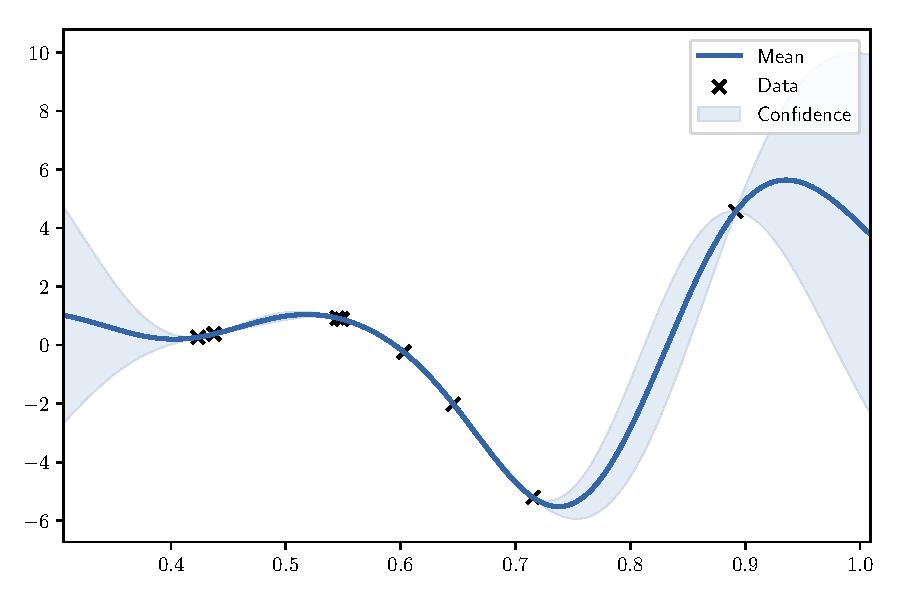
\includegraphics[width=0.5\textwidth]{gp_first_example.pdf} 
\end{center}
\end{frame}

\begin{frame}{The scaling behavior w.r.t. $N$}
The computational cost of Gaussian process is $O(N^3)$.
\begin{center}
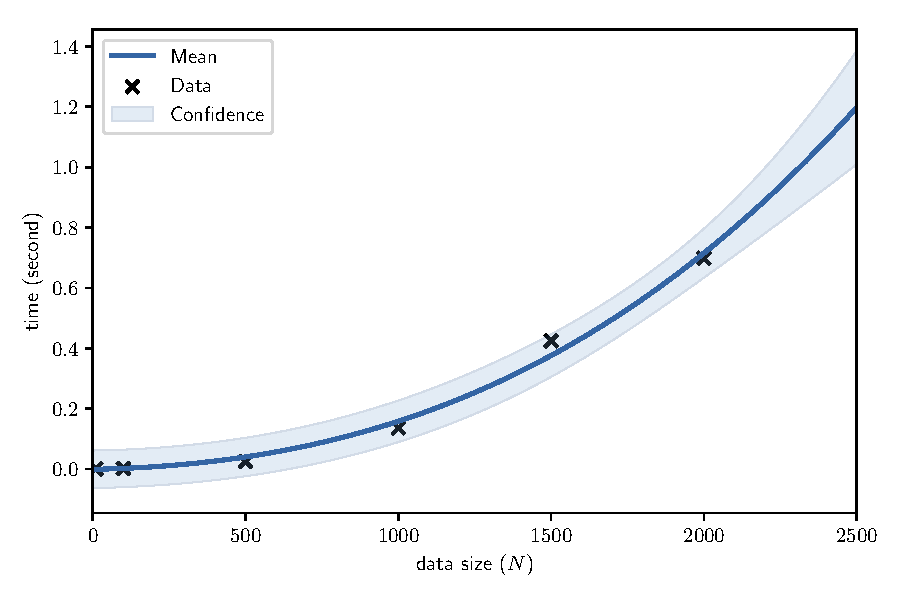
\includegraphics[width=0.6\textwidth]{gp_scaling.pdf} 
\end{center}
\end{frame}

\begin{frame}{Behind a Gaussian process fit}
\begin{itemize}

\item Point Estimate / Maximum A Posteriori (MAP) of hyper-parameters.
%
\[
\theta^* = \argmax_{\theta} \log p(\yV|\xM, \theta) = \argmax_{\theta} \log \gaussianDist{\yV}{0}{\K+\sigma^2\I}
\]

\item Prediction on a test point given the observed data and the optimized hyper-parameters.
\begin{align*}
p(\fV_* | &\xM_*, \yV, \xM, \theta) = \\
& \gaussianDist{\fV_*}{\K_* (\K+\sigma^2\I)^{-1} \yV}{\K_{**} - \K_* (\K+\sigma^2\I)^{-1} \K_*^\top}
\end{align*}

\end{itemize}
\end{frame}

\begin{frame}{How to implement the log-likelihood (1)}
\begin{itemize}
\item Compute the covariance matrix $\K$:
\[\K = 
 \begin{pmatrix}
  k(\xV_1, \xV_1) & \cdots & k(\xV_1, \xV_N) \\
  \vdots  &  \ddots & \vdots  \\
  k(\xV_N, \xV_1) & \cdots & k(\xV_N, \xV_N) 
 \end{pmatrix}
 \]
where $k(\xV_i, \xV_j) = \gamma \exp\left(-\frac{1}{2l^2}(\xV_i - \xV_j)^\top(\xV_i - \xV_j)\right)$
\vspace{5mm}
\item The complexity is $O(N^2Q)$.
\end{itemize}
\end{frame}

\begin{frame}{How to implement the log-likelihood (2)}
\begin{itemize}
\item Plug in the log-pdf of multi-variate normal distribution:
\begin{align*}
\log p(\yV|\xM) =&  \log \gaussianDist{\yV}{0}{\K+\sigma^2\I}\\
=& -\frac{1}{2}\log |2\pi (\K+\sigma^2\I)| - \frac{1}{2} \yV^\top (\K+\sigma^2\I)^{-1} \yV\\
=& -\frac{1}{2}(||\L^{-1}\yV||^2+N\log 2\pi)-\sum_i \log \L_{ii}
\end{align*}
\item Take a Cholesky decomposition: $\L = \mathtt{chol}(\K+\sigma^2\I )$.
\item The computational complexity is $O(N^3 + N^2 + N)$. Therefore, the overall complexity including the computation of $\K$ is $O(N^3)$.
\end{itemize}
\end{frame}

%\begin{frame}{How to implement the log-likelihood (3)}
%\begin{align*}
%\log p(\yV|\xM) =& -\frac{1}{2}\log |2\pi (\K+\sigma^2\I)| - \frac{1}{2} \yV^\top (\K+\sigma^2\I)^{-1} \yV\\
%=& -\frac{1}{2}\log \left((2\pi)^N |\L\L^\top|\right) - \frac{1}{2} \tr{\yV^\top (\L\L^\top)^{-1} \yV} \\
%=& -\frac{N}{2}\log 2\pi  -\log  |\L|- \frac{1}{2} \tr{(\L^{-1}\yV)^\top \L^{-1}\yV} \\
%=& -\frac{1}{2}(||\L^{-1}\yV||^2+N\log 2\pi)-\sum_i \log \L_{ii}
%\end{align*}
%The computational complexity is $O(N^3 + N^2 + N)$. Therefore, the overall complexity including the computation of $\K$ is $O(N^3)$.
%\end{frame}

\begin{frame}[fragile]{A quick profiling ($N$=1000, $Q$=10)}
Time unit is microsecond.
\small
\begin{verbatim}
Line #     Time    % Time     Line Contents
 2                        def log_likelihood(kern, X, Y, sigma2):
 3          6.0      0.0      N = X.shape[0]
 4      55595.0     58.7      K = kern.K(X)
 5       4369.0      4.6      Ky = K + np.eye(N)*sigma2
 6      30012.0     31.7      L = np.linalg.cholesky(Ky)
 7       4361.0      4.6      LinvY = dtrtrs(L, Y, lower=1)[0]
 8         49.0      0.1      logL = N*np.log(2*np.pi)/-2.
 9         82.0      0.1      logL += np.square(LinvY).sum()/-2.
10        208.0      0.2      logL += -np.log(np.diag(L)).sum()
11          2.0      0.0      return logL
\end{verbatim}
\end{frame}

\begin{frame}{Too slow or too many data points?}
A lot of data does not necessarily mean a complex model.
\begin{center}
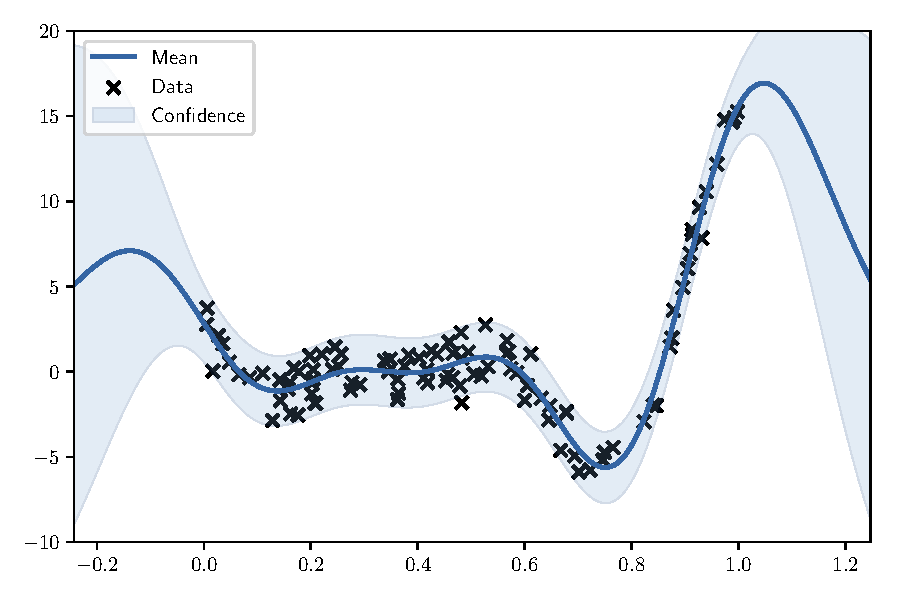
\includegraphics[width=0.8\textheight]{gp_example_lots_data.pdf} 
\hfill
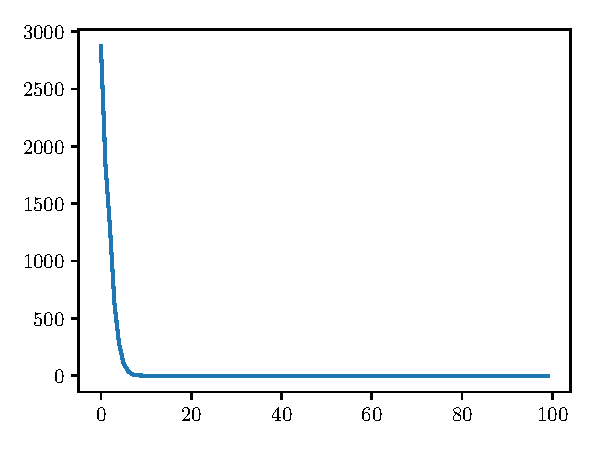
\includegraphics[width=0.74\textheight]{lots_data_eigen_values.pdf} 
\end{center}
\end{frame}

\begin{frame}{Pseudo Data}
Summarize \textit{real} data into a small set of \textit{pseudo} data.
\begin{center}
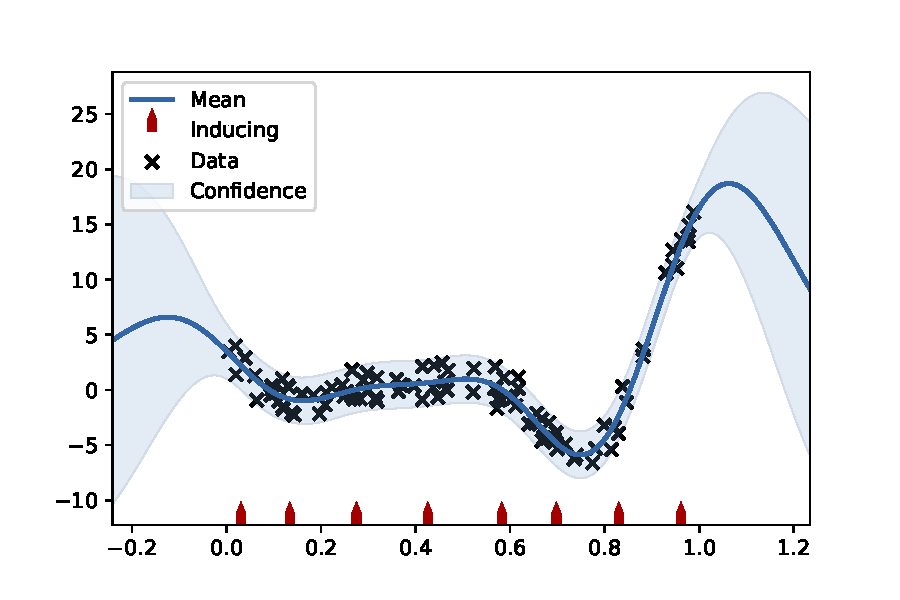
\includegraphics[width=0.6\textwidth]{sparsegp_example_lots_data.pdf} 
\end{center}
\end{frame}

\begin{frame}{Sparse Gaussian Process}
Sparse GPs refers to a family of approximations:
\begin{itemize}
\item Nystr\"{o}m approximation \citep{WilliamsSeeger2001}
\item Fully independent training conditional (FITC) \citep{SnelsonZoubin2006}
\item Variational sparse Gaussian process \citep{Titsias2009}
\end{itemize}
\end{frame}

\begin{frame}{Approximation by subset}
\begin{itemize}
\item Let's randomly pick a subset from the training data: $\zM \in \R^{M\times Q}$.
\item Approximate the covariance matrix $\K$ by $\tilde{\K}$.
\vspace{5mm}

$\tilde{\K} = \K_z \K_{zz}^{-1} \K_z^\top$, where $\K_{z} = \K(\xM, \zM)$ and $\K_{zz} = \K(\zM, \zM)$.
\vspace{5mm}
\item Note that $\tilde{\K} \in \R^{N\times N}$, $\K_{z} \in \R^{N\times M}$ and $\K_{zz} \in \R^{M \times M}$.
\item The log-likelihood is approximated by 
\[
\log p(\yV|\xM, \theta) \approx  \log \gaussianDist{\yV}{0}{\K_z \K_{zz}^{-1} \K_z^\top+\sigma^2\I}.
\]
\end{itemize}
\end{frame}

\begin{frame}{Efficient computation using Woodbury formula}
\begin{itemize}
\item The naive formulation does not bring any computational benefits.
\[
\tilde{\bound} = -\frac{1}{2}\log |2\pi (\tilde{\K}+\sigma^2\I)| - \frac{1}{2} \yV^\top (\tilde{\K}+\sigma^2\I)^{-1} \yV
\]
\item Apply the Woodbury formula:
\[
(\K_z \K_{zz}^{-1} \K_z^\top+\sigma^2\I)^{-1} = \sigma^{-2}\I - \sigma^{-4} \K_z (\K_{zz} + \sigma^{-2}\K_z^\top\K_z)^{-1}\K_z^\top
\]
\item Note that $(\K_{zz} + \sigma^{-2}\K_z^\top\K_z) \in \R^{M \times M}$.
\item The computational complexity reduces to $O(NM^2)$.
\end{itemize}
\end{frame}

\begin{frame}{Nystr\"{o}m approximation}
\begin{itemize}
\item The above approach is called Nystr\"{o}m approximation by \cite{WilliamsSeeger2001}.
\item The approximation is directly done on the covariance matrix without the concept of pseudo data.
\item The approximation becomes exact if the whole data set is taken, \ie $\K \K^{-1} \K^\top = \K$.
\item The subset selection is done randomly.
\end{itemize}
\end{frame}

\begin{frame}{Gaussian process with Pseudo Data (1)}
\begin{itemize}
\item \cite{SnelsonZoubin2006} proposes the idea of having pseudo data. This approach is later referred to as  
Fully independent training conditional (FITC).
\item Augment the training data ($\xM$, $\yV$) with pseudo data $\uV$ at location $\zM$.
\begin{align*}
p\left(\begin{bmatrix}
\yV \\ \uV \end{bmatrix}|\begin{bmatrix}
\xM \\ \zM \end{bmatrix} \right) =&  \gaussianDist{\begin{bmatrix}
\yV \\ \uV \end{bmatrix}}{0}{\begin{bmatrix}
\K_{ff}+\sigma^2\I & \K_{fu}  \\ \K_{fu}^\top & \K_{uu} \end{bmatrix}}
\end{align*}
where $\K_{ff} = \K(\xM, \xM)$, $\K_{fu} = \K(\xM, \zM)$ and $\K_{uu} = \K(\zM, \zM)$.
\end{itemize}
\end{frame}

\begin{frame}{Gaussian process with Pseudo Data (2)}
\begin{itemize}
\item Thanks to the marginalization property of Gaussian distribution,
\[
p(\yV| \xM) = \int_{\uV} p(\yV, \uV | \xM, \zM).
\]
\item Further re-arrange the notation:
\begin{align*}
p(\yV, \uV| \xM, \zM) = p(\yV| \uV, \xM, \zM) p(\uV| \zM)
\end{align*}
where $p(\uV| \zM) = \gaussianDist{\uV}{0}{\K_{uu}}$, 
$p(\yV| \uV, \xM, \zM)=\gaussianDist{\yV}{\K_{fu} \K_{uu}^{-1} \uV}{\K_{ff} - \K_{fu} \K_{uu}^{-1} \K_{fu}^\top+\sigma^2\I}$.
\end{itemize}
\end{frame}

\begin{frame}{FITC approximation (1)}
\begin{itemize}
\item So far, $p(\yV | \xM)$ has not been changed, but there is no speed-up, $\K_{ff} \in \R^{N\times N}$ in $\K_{ff} - \K_{fu} \K_{uu}^{-1} \K_{fu}^\top+\sigma^2\I$.

\item The FITC approximation assumes
\[
\tilde{p}(\yV| \uV, \xM, \zM)=\gaussianDist{\yV}{\K_{fu} \K_{uu}^{-1} \uV}{\lambdaM +\sigma^2\I},
\]
where $\lambdaM = (\K_{ff} - \K_{fu} \K_{uu}^{-1} \K_{fu}^\top)\circ \I$.
\end{itemize}
\end{frame}

\begin{frame}{FITC approximation (2)}
\begin{itemize}
\item Marginalize $\uV$ from the model definition:
\[
\tilde{p}(\yV| \xM, \zM) = \gaussianDist{\yV}{0}{\K_{fu} \K_{uu}^{-1} \K_{fu}^\top+\lambdaM +\sigma^2\I}
\]

\item Woodbury formula can be applied in the sam way as in Nystr\"{o}m approximation:
\[
(\K_z \K_{zz}^{-1} \K_z^\top+\lambdaM+\sigma^2\I)^{-1} = \aM - \aM \K_z (\K_{zz} + \K_z^\top\aM\K_z)^{-1}\K_z^\top\aM,
\]
where $\aM = (\lambdaM+\sigma^2\I)^{-1}$.
\end{itemize}
\end{frame}

\begin{frame}{FITC approximation (3)}
\begin{itemize}
\item FITC allows the pseudo data not being a subset of training data.

\item The inducing inputs $\zM$ can be optimized via gradient optimization.

\item Like Nystr\"{o}m approximation, when taking all the training data as inducing inputs, the FITC approximation is equivalent to the original GP:
\[
\tilde{p}(\yV| \xM, \zM=\xM) = \gaussianDist{\yV}{0}{\K_{ff} +\sigma^2\I}
\]
\item FITC can be combined easily with expectation propagation (EP). \cite{BuiEtAl2017} provides an overview and a nice connection with variational sparse GP.
\end{itemize}
\end{frame}

\begin{frame}{Model Approximation vs. Approximate Inference}
When the exact model/inference is intractable, typically there are two types of approaches:
\begin{itemize}
\item Approximate the original model with a simpler one such that inference becomes tractable, like Nystr\"{o}m approximation, FITC.
\item Keep the original model but derive an approximate inference method which is often \textit{not} able to return the true answer, like variational inference.
\end{itemize}

\end{frame}

\begin{frame}{Model Approximation vs. Approximate Inference}
A problem with model approximation is that 
\begin{itemize}
\item when an approximated model requires some tuning, e.g., for hyper-parameters, it is unclear how to improve it based on training data.

\item In the case of FITC, we know the model is correct if $\zM = \xM$, however, optimizing $\zM$ will not necessarily lead to a better location.

\item In fact, optimizing $\zM$ can lead to overfitting. \citep{QuinoneroRasmussen2005}
\end{itemize}

\end{frame}

\begin{frame}{Variational Sparse Gaussian Process (1)}

\begin{itemize}
\item \cite{Titsias2009} introduces a variational approach for sparse GP.
\item It follows the same concept of pseudo data:
\begin{align*}
p(\yV| \xM) = \int_{\fV, \uV} p(\yV| \fV) p(\fV| \uV, \xM, \zM) p(\uV| \zM)
\end{align*}
where $p(\uV| \zM) = \gaussianDist{\uV}{0}{\K_{uu}}$, 
$p(\yV| \uV, \xM, \zM)=\gaussianDist{\yV}{\K_{fu} \K_{uu}^{-1} \uV}{\K_{ff} - \K_{fu} \K_{uu}^{-1} \K_{fu}^\top+\sigma^2\I}$.

\end{itemize}
\end{frame}

\begin{frame}{Variational Sparse Gaussian Process (2)}
\begin{itemize}
\item Instead of approximate the model, \cite{Titsias2009} derives a variational lower bound.

\item Normally, a variational lower bound of a marginal likelihood, also known as evidence lower bound (ELBO), looks like
\begin{align*}
\log p(\yV | \xM) =& \log \int_{\fV, \uV} p(\yV | \fV) p(\fV| \uV, \xM, \zM) p(\uV | \zM) \\
\geq& \int_{\fV, \uV} q(\fV, \uV) \log \frac{p(\yV | \fV) p(\fV| \uV, \xM, \zM) p(\uV | \zM)}{q(\fV, \uV)}.
\end{align*}
\end{itemize}

\end{frame}

\begin{frame}{\textit{Special} Variational Posterior}
\begin{itemize}
\item \cite{Titsias2009} defines an unusual variational posterior:
\[
q(\fV, \uV) = p(\fV| \uV, \xM, \zM) q(\uV), \quad \text{where } q(\uV) = \gaussianDist{\uV}{\mu}{\Sigma}.
\]
\item Plug it into the lower bound:
\begin{align*}
\bound =& \int_{\fV, \uV} p(\fV| \uV, \xM, \zM) q(\uV) \log \frac{p(\yV | \fV) \cancel{p(\fV| \uV, \xM, \zM)} p(\uV | \zM)}{\cancel{p(\fV| \uV, \xM, \zM)} q(\uV)} \\
=& \expectation{\log p(\yV | \fV)}_{p(\fV| \uV, \xM, \zM) q(\uV)} - \KL{q(\uV)}{p(\uV|\zM)}\\
=& \expectation{\log \gaussianDist{\yV}{\K_{fu}\K_{uu}^{-1}\uV}{\sigma^2\I}}_{q(\uV)} - \KL{q(\uV)}{p(\uV|\zM)}
\end{align*}

\end{itemize}
\end{frame}

\begin{frame}{\textit{Special} Variational Posterior}
\begin{itemize}
\item There is no inversion of any big covariance matrices in the first term:
\begin{align*}
 -\frac{N}{2}\log 2\pi \sigma^2 -\frac{1}{2\sigma^2}\expectation{(\K_{fu}\K_{uu}^{-1}\uV-\yV)^\top(\K_{fu}\K_{uu}^{-1}\uV-\yV)}_{q(\uV)}
\end{align*}
\item The overall complexity of the lower bound is $O(NM^2)$.
\end{itemize}
\end{frame}

\begin{frame}{Tighten the Bound}
\begin{itemize}
\item Find the optimal parameters of $q(\uV)$:
\[
\mu^*, \Sigma^* = \argmax_{\mu, \Sigma} \bound(\mu, \Sigma).
\]
\item Make the bound as tight as possible by plugging in $\mu^*$ and $\Sigma^*$:
\[
\bound = \log \gaussianDist{\yV}{0}{\K_{fu} \K_{uu}^{-1} \K_{fu}^\top+ \sigma^2\I} - \frac{1}{2\sigma^2}\tr{\K_{ff} - \K_{fu} \K_{uu}^{-1} \K_{fu}^\top}.
\]
\item The overall complexity of the lower bound remains $O(NM^2)$.
\end{itemize}
\end{frame}

\begin{frame}{Variational sparse GP}
\begin{itemize}
\item Note that $\bound$ is not a valid log-pdf, $\int_{\yV} \exp(\bound(\yV)) \leq 1$, due to the trace term.
\item As inducing points are variational parameters, optimizing the inducing inputs $\zM$ always leads to a better bound.
\item The model does not ``overfit" with too many inducing points. 
\end{itemize}
\vspace{-5mm}
\begin{center}
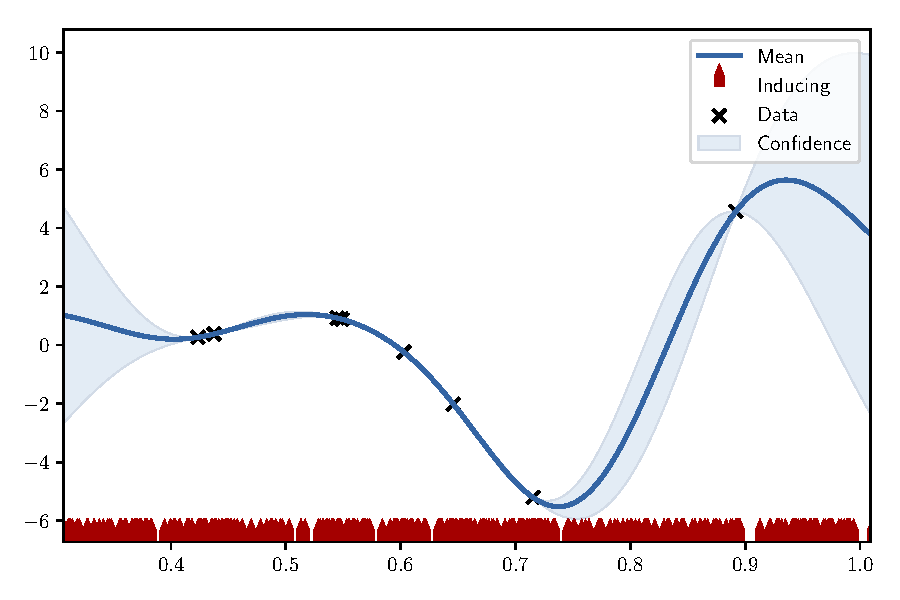
\includegraphics[width=0.5\textwidth]{sparsegp_example_lots_inducing_points.pdf} 
\end{center}
\end{frame}

\begin{frame}{An alternative view of sparse GP}
Is variational sparse GP a \textit{hack} only working for GP?
\end{frame}

\begin{frame}{The two key ingredients}
The two key ingredients of variational sparse GP:
\begin{itemize}
\item Variational compression \citep{HensmanLawrence2014}
\item Variational posterior with ``pseudo data" (``variational Gaussian process" by \cite{TranEtAl2016})
\end{itemize}
\end{frame}

\begin{frame}{A generic variational lower bound}
Consider a generic probabilistic model $p(y| h) p(h |x)$ with $h$ being a latent variable. A variational lower bound is typically like
\begin{align*}
\log p(y | x) \geq& \int_{h} q(h) \log \frac{p(y| h) p(h |x)}{q(h)}
\end{align*}
\end{frame}

\begin{frame}{Use prior as posterior}

We are free to choose the form of the variational posterior. It is always possible to choose $q(h) = p(h|x)$.
This results into a lower bound:
\begin{align*}
\bound = \int_h p(h|x) \log p(y|h).
\end{align*}
The same idea can be easily applied to a deeper model:
\begin{align*}
\log p(y | x) =& \log \int_{h_1, h_2, h_3} p(y| h_1) p(h_1|h_2) p(h_2 | h_3) p(h_3 |x ) \\
\geq& \int_{h_1, h_2, h_3} p(h_1|h_2) p(h_2 | h_3) p(h_3 |x ) \log p(y|h_1)
\end{align*}
This is weird. Does it work?
\end{frame}

\begin{frame}{Sigmoid Belief Networks}
It works surprising well. \cite{DaiLawrence2015} applied this trick to sigmoid belief networks (SBN):
\[
p(\yV|\hV_{1}) \prod_{l=1}^{L-1} p(\hV_{l}|\hV_{l+1}) p(\hV_L),
\]
where
\begin{align*}
p(\yV|\hV_{1}) =& \prod_i \sigma(\wM_{1,i}\hV_{1}+\bV_{1,i})^{y_i}\sigma(-\wM_{1,i}\hV_{1}-\bV_{1,i})^{1-y_i},\\ 
 p(\hV_l|\hV_{l+1}) =& \prod_i \sigma(\wM_{l+1,i}\hV_{l+1}+\bV_{l+1,i})^{h_{l,i}}\sigma(-\wM_{l+1,i}\hV_{l+1}-\bV_{l+1,i})^{1-h_{l,i}}\\
 p(\hV_L) =& \prod_{i} \pi_i^{h_{Li}}(1-\pi_i)^{1-h_{Li}}
\end{align*}

\begin{align*}
\bound = \int_{\hV_1, \ldots, \hV_L} q(\hV_L) \prod_{l=1}^{L-1} p(\hV_l|\hV_{l+1}) \log p(\yV|\hV_1)
\end{align*}
\end{frame}

\begin{frame}{Sigmoid Belief Networks}
Variational Inference of SBN is very hard \citep{MnihGregor2014}:
\[
\log p(\yV) \geq \sum_{\hV_1, \ldots, \hV_L} q(\hV_1, \ldots, \hV_L) \log \frac{p(\yV|\hV_{1}) \prod_{l=1}^{L-1} p(\hV_{l}|\hV_{l+1}) p(\hV_L)}{q(\hV_1, \ldots, \hV_L)}
\]

\begin{align*}
\bound = \sum_{\hV_1, \ldots, \hV_L} q(\hV_L) \prod_{l=1}^{L-1} p(\hV_l|\hV_{l+1}) \log p(\yV|\hV_1)
\end{align*}
\end{frame}

\begin{frame}
\begin{columns}

\begin{column}[t]{0.3\linewidth}
\footnotesize
\vspace{1cm}
\begin{itemize}
\item 3 hidden layers (100-100-10)
\item the generated examples from each value in the top layer
\item in total 1024 examples
\item columns encode first 5 bits.
\item rows encode later 5 bits.
\end{itemize}
\end{column}
\hfill
\begin{column}[t]{0.68\linewidth}
\begin{center}
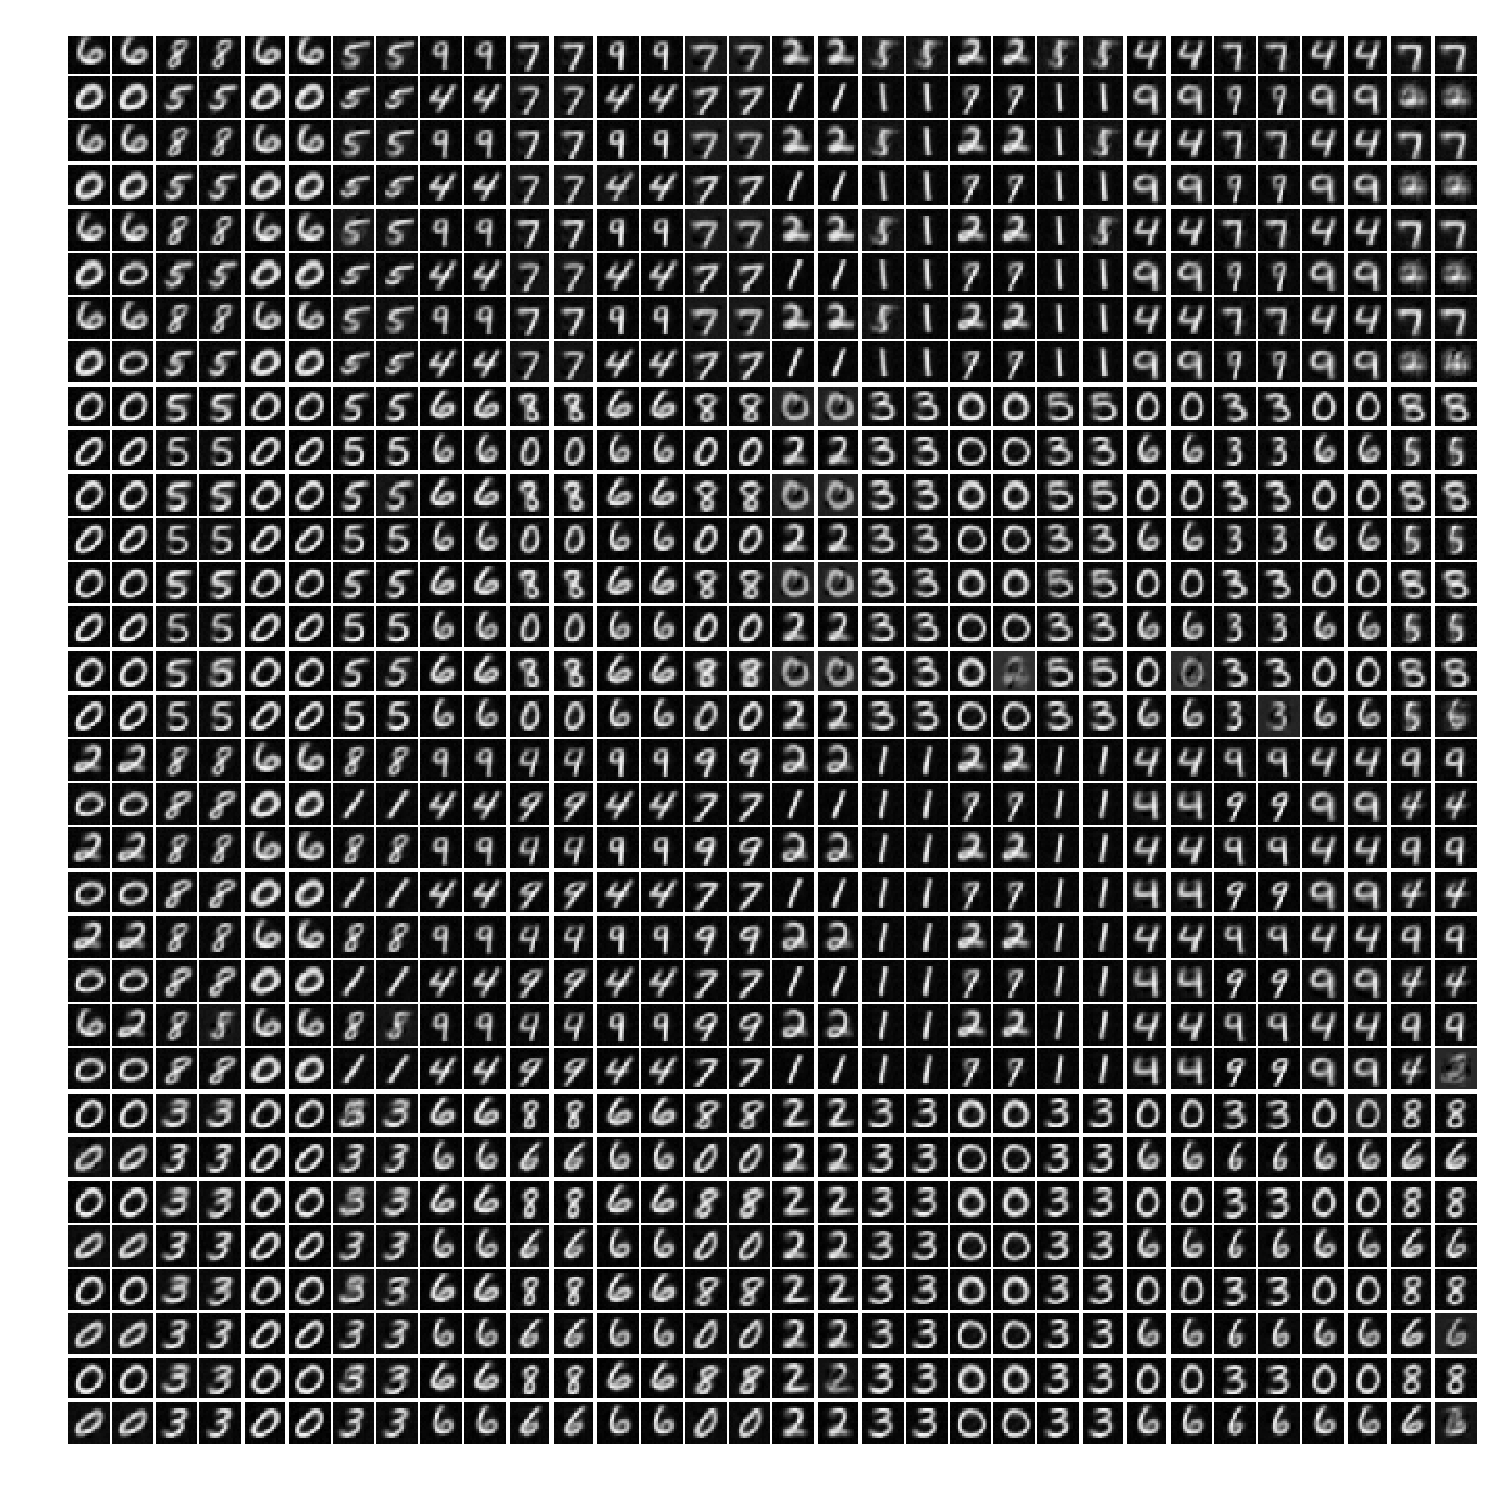
\includegraphics[width=0.95\textheight]{varsbn_mnist.pdf} 
\end{center}
\end{column}
\end{columns}
\end{frame}

\begin{frame}{What is the price?}
The variational lower bound can also be written as
\begin{align*}
\log p(y | x) = \int_{h} q(h) \log \frac{p(y| h) p(h |x)}{q(h)} + \KL{q(h)}{p(h|x, y)}
\end{align*}

With $q(h) = p(h|x)$,
\begin{align*}
\log p(y | x) = \int_{h} p(h|x) \log p(y| h) + \KL{p(h|x)}{p(h|x, y)}
\end{align*}
\end{frame}

\begin{frame}{What is the price?}
The lower bound is exact \textit{only if} the posterior is same as the prior.

\begin{align*}
\log p(y | x) = \int_{h} p(h|x) \log p(y| h) + \KL{p(h|x)}{p(h|x, y)}
\end{align*}
\vspace{-5mm}
\[
p(h|x, y) = \frac{p(y|h) p(h|x)}{\int_{h'} p(y|h') p(h'|x)}
\]
\vspace{-5mm}
$\KL{p(h|x)}{p(h|x, y)}$ is zero, when
\begin{itemize}
\item $y$ is independent of $h$, i.e., $p(y|h) = p(y)$.
\item $p(h|x)$ is a deterministic relation, i.e., $p(h|x) = \delta(h(x))$.
\end{itemize}
\end{frame}

\begin{frame}{A bias towards being a deterministic function}
This variational posterior introduces a bias towards being a deterministic function.

Assume the model is parameterized by $\theta$, i.e., $p(y|h, \theta) p(h|x, \theta)$.

Point Estimate: 
\begin{align*}
\theta^* = \argmax_{\theta} \bound(\theta) = \argmax_{\theta}  \left( \log p(y | x, \theta) - \KL{p(h|x, \theta)}{p(h|x, y, \theta)} \right)
\end{align*}
\end{frame}

\begin{frame}{A bias towards being a deterministic function}
Variational Inference:
\begin{align*}
\hat{\bound} =& \int_{h, \theta} p(h|x, \theta) q(\theta) \log \frac{p(y|h, \theta) \cancel{p(h|x,\theta)} p(\theta)}{\cancel{p(h|x, \theta)} q(\theta)} \\
=& \expectation{\log p(y | x, \theta) - \KL{p(h|x, \theta)}{p(h|x, y, \theta)}}_{q(\theta)} - \KL{q(\theta)}{p(\theta)} \\
=& \expectation{\log p(y | x, \theta)}_{q(\theta)} - \KL{q(\theta)}{p(\theta)} \\
& - \expectation{\KL{p(h|x, \theta)}{p(h|x, y, \theta)}}_{q(\theta)}
\end{align*}
\end{frame}

\begin{frame}{The bias in variational Sparse GP}
Variational sparse GP often "under-fit".
\begin{align*}
\bound =& \int_{\fV, \uV} p(\fV| \uV, \xM, \zM) q(\uV) \log \frac{p(\yV | \fV) \cancel{p(\fV| \uV, \xM, \zM)} p(\uV | \zM)}{\cancel{p(\fV| \uV, \xM, \zM)} q(\uV)} \\
=& \int_{\fV, \uV} p(\fV| \uV, \xM, \zM) q(\uV) \log p(\yV | \fV)  - \KL{q(\uV)}{p(\uV| \zM)}\\
=& \expectation{\log p(\yV | \xM, \uV, \zM)}_{q(\uV)} - \KL{q(\uV)}{p(\uV| \zM)} \\
& - \expectation{\KL{p(\fV|\xM, \uV, \zM)}{p(\fV|\xM, \yV, \uV, \zM)}}_{q(\uV)}
\end{align*}
\end{frame}

\begin{frame}{Flexible variational posterior}
Consider a generic probabilistic model, e.g., $p(\yV | \fV) p(\fV)$.

Variational lower bound:
\[
\bound = \int_{\fV} q(\fV) \log \frac{p(\yV | \fV) p(\fV)}{q(\fV)}
\]

One flexible variational posterior:
\[
q(\fV) = \int_{\fV} q(\fV|\uV) q(\uV)
\]
\end{frame}

\begin{frame}{Auxiliary variable}
It may not be tractable to compute $ \int_{\fV} q(\fV|\uV) q(\uV)$.

One way to work around is to introduce $\uV$ as an auxiliary variable to the model:
\[
p(\yV | \fV) p(\fV) p(\uV|\fV)
\]
Note that we are free to choose the form of $p(\uV|\fV)$ and $q(\uV)$ and $q(\fV|\uV)$.
\end{frame}

\begin{frame}{A further lower bound}
show the relation between two lower bounds.
\begin{align*}
\int_{\fV} q(\fV) \log \frac{p(\yV | \fV) p(\fV)}{q(\fV)} =& \int_{\fV, \uV}q(\uV|\fV) q(\fV) \log \frac{p(\yV | \fV) p(\fV) p(\uV|\fV) }{q(\uV|\fV) q(\fV)} \\
& -  \int_{\fV} q(\fV) \int_{\uV} q(\uV|\fV)  \log \frac{p(\uV|\fV) }{q(\uV|\fV)}
\end{align*}

\begin{align*}
\bound = \bound_{\fV, \uV}  - \expectation{\KL{q(\uV|\fV)}{p(\uV|\fV)}}_{ q(\fV)} \geq \bound_{\fV, \uV}
\end{align*}
\end{frame}


\begin{frame}{In the case of spare GP}
This leads back to the usual sparse GP bound that we know.
\begin{align*}
p(\yV| \fV) &= \gaussianDist{\yV}{\fV}{\sigma^2 \I} \\ 
p (\fV| \xM) &= \gaussianDist{\fV}{0}{\K(\xM, \xM)} \\
p(\uV| \zM, \fV, \xM) &= \gaussianDist{\uV}{\K_{uf} \K_{ff}^{-1}\fV}{\K_{uu} - \K_{fu}^\top \K_{ff}^{-1} \K_{fu}} \\
q(\uV | \fV) q(\fV) &= q(\fV | \uV) q(\uV) = p(\fV|\xM, \uV, \zM) q(\uV)
\end{align*}
\end{frame}

%\begin{frame}{$\zM$ is a variational parameter!}
%The variational sparse GP model is $p(\yV|\fV) p(\fV|\xM, \uV, \zM) p(\uV| \zM)$ with $\uV$ being latent variable. Why $\zM$ is a variational parameter?
%\end{frame}

\begin{frame}{Parallel Sparse Gaussian Process}
\begin{itemize}
\item Beyond Approximate the inference method, maybe we could exploit parallelization.
\item For Gaussian process, it turns out to be very hard, because parallel Cholesky decomposition is very difficult.
\item \cite{DaiEtAl2014} and \cite{GalEtAl2014} proposes a parallel inference method for sparse GP.
\end{itemize}
\end{frame}

\begin{frame}{Data Parallelism}
\begin{itemize}
\item Consider a training set: $\mathcal{D} = \{(\xV_1, y_1), \ldots,  (\xV_N, y_N)\}$.
\item Assume there are $C$ computational cores/machines.
\item A data parallelism algorithm divides the data set into $C$ partitions as evenly as possible: $\mathcal{D} = \bigcup_{c=1}^C \mathcal{D}_c$.
\item The parallelism happens in the way that the function running on each core only requiring the data from the local partition.
\end{itemize}
\end{frame}

\begin{frame}{A simple example: neural network regression}
\begin{align*}
l = \sum_{n=1}^N ||y_n - f_\theta( \xV_n )||^2 = \sum_{c=1}^C \sum_{n_c \in \mathcal{D}_c} ||y_{n_c} -  f_\theta( \xV_{n_c} )||^2
\end{align*}
\vspace{-10mm}
\begin{enumerate}
\item Each core computes its local objective $l_c = \sum_{n_c \in \mathcal{D}_c} ||y_{n_c} -  f_\theta( \xV_{n_c} )||^2$.
\item Each core computes the gradient of its local object $\partial l_c/ \partial \theta$.
\item Aggregate all the local objectives and gradients $l = \sum_{c=1}^C l_c$ and $\partial l/ \partial \theta = \sum_{c=1}^C \partial l_c/ \partial \theta$.
\item Take a step along the gradient following a gradient descent algorithm.
\item Repeat Step 1 until converge.
\end{enumerate}
\end{frame}

\begin{frame}{Data Parallelism for Sparse GP}
The variational lower bound (after applying Woodbury formula) is
\begin{align*}
\bound =& -\frac{N}{2}\log 2\pi \sigma^2 +\frac{1}{2} \log \frac{|\K_{uu}|}{|\K_{uu}+\sigma^{-2}\phiM|} -\frac{1}{2\sigma^2}\yV^\top\yV\\
&+\frac{1}{2\sigma^4}\yV^\top\K_{fu}(\K_{uu} + \phiM)^{-1}\K_{fu}^\top\yV - \frac{1}{2\sigma^2}\phiV +  \frac{1}{2\sigma^2}\tr{\K_{uu}^{-1}\phiM}
\end{align*}
where $\phiM = \K_{fu}^\top \K_{fu}$ and $\phiV = \tr{\K_{ff}}$.
\end{frame}

\begin{frame}{Data Parallelism for Sparse GP}
\begin{itemize}
\item The lower bound is not fully distributable like in the simple example.
\item All the terms involving data can be written as a sum across data points:
\begin{align*}
&\yV^\top\yV = \sum_{n=1}^N y_n^2, \quad \yV^\top\K_{fu} = \sum_{n=1}^N y_n \K_{f_n u}, \quad \phiM = \sum_{n=1}^N \K_{f_n u}^\top \K_{f_n u}\\
&\phiV = \sum_{n=1}^N\K_{f_n f_n}, \text{where } \K_{f_n u} = \K(\xV_n, \zM), \quad \K_{f_n f_n} = \K(\xV_n, \xV_n).
\end{align*}
\end{itemize}
\end{frame}

\begin{frame}{Data Parallelism for Sparse GP}
\begin{enumerate}
\item \textbf{[local]} Compute all the data related terms locally: $\yV_c^\top\yV_c$, $\yV_c^\top\K_{f_c u}$, $\phiM_c$ and $\phiV_c$.
\item \textbf{[global]} Aggregate all the local terms and compute the lower bound $\bound$ on one node.
\item \textbf{[global]} Compute the gradient of the bound w.r.t. the model parameters.
\item \textbf{[global]} Compute the gradient w.r.t. the local terms $\partial \bound/\partial \K_{f_c u}$, $\partial \bound/\partial \phiM_c$ and $\partial \bound/\partial \phiV_c$ and broadcast to individual nodes.
\item \textbf{[local]} Compute the gradient contribution of the local terms and aggregate the local gradients into the final gradient.
\item \textbf{[global]} Take a gradient step and repeat Step 1.
\end{enumerate}
\end{frame}

\begin{frame}{Data Parallelism for Sparse GP}
\begin{center}
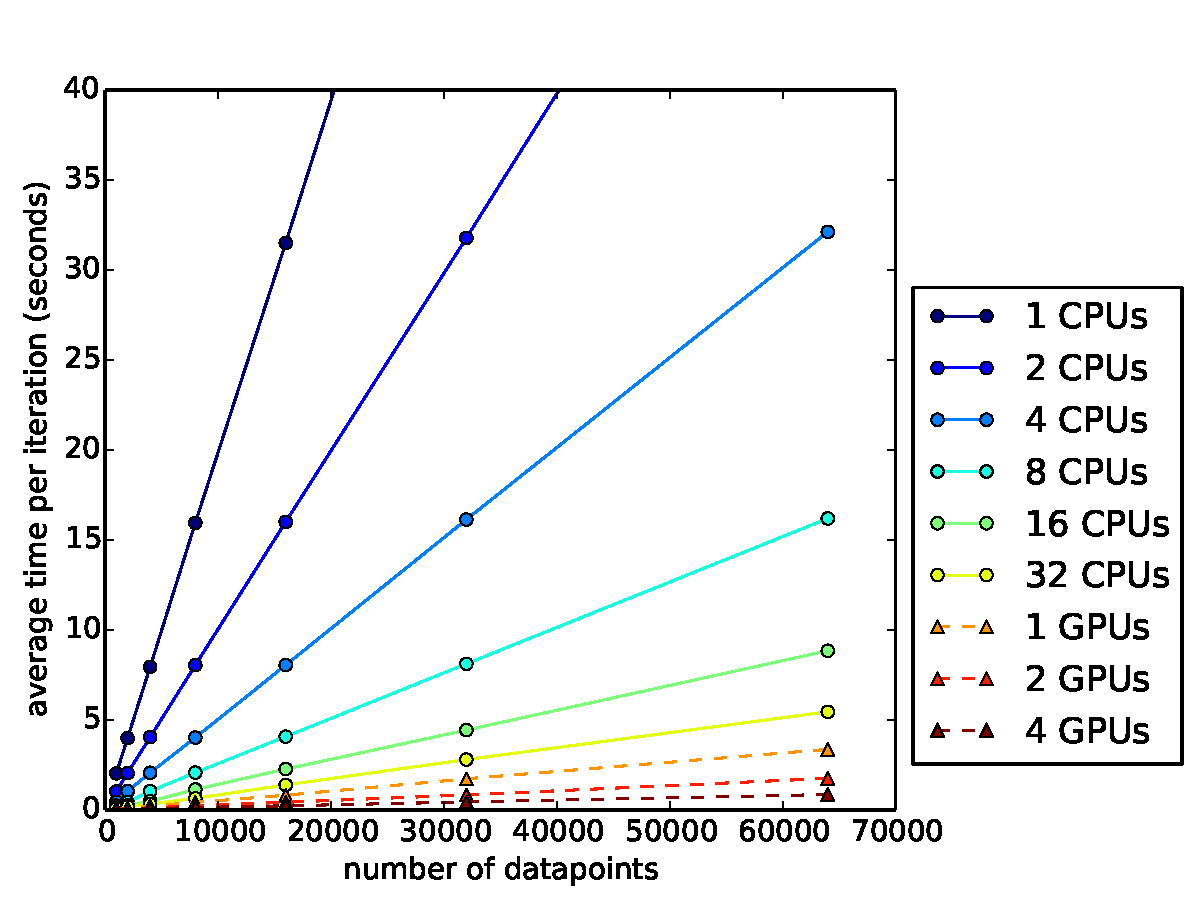
\includegraphics[width=0.48\textwidth]{parallel_scaling.pdf} 
\hfill
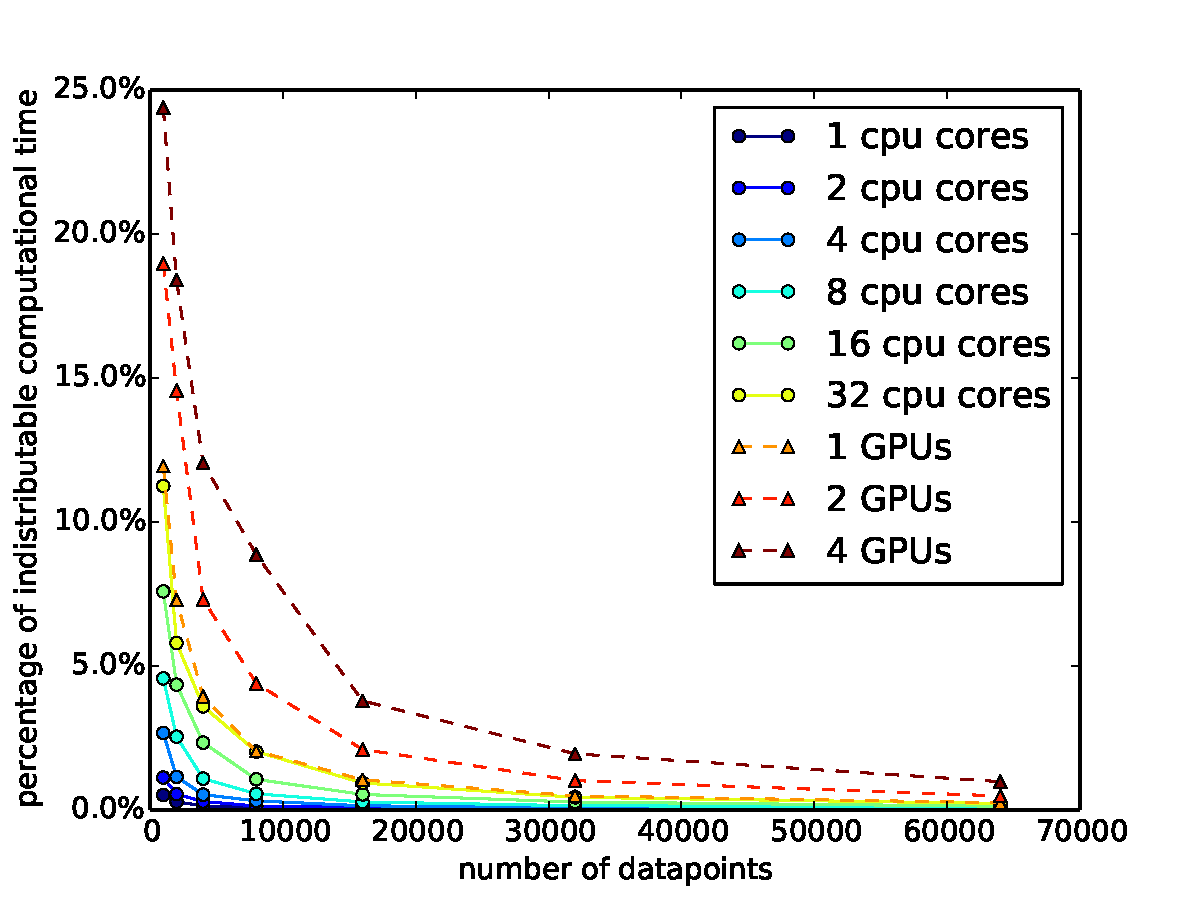
\includegraphics[width=0.48\textwidth]{parallel_portion.pdf} 
\end{center}
\end{frame}

%\begin{frame}{Stochastic variational Gaussian process}
%\end{frame}

%\begin{frame}{Distributed Gaussian Processes}
%\end{frame}

\begin{frame}{The emerge of deep learning platforms}
\begin{itemize}
\item Deep learning platforms such as Theano, Tensorflow, Torch, Caffe, MXNet emerge in recent years.
\item It standardizes deep neural networks programming.
\item Auto-differentiation enables the flexible construction of DNNs.
\item GPU acceleration enables scalability for real world applications.
\end{itemize}
\end{frame}

\begin{frame}{GPU for machine learning}
\begin{columns}
\begin{column}[t]{0.6\linewidth}
\small
\begin{itemize}
\item Von Neumann architecture is not suitable for machine learning.
\item Memory bandwidth: \\
GPU(NVidia V100, AWS P3): 900 GB/s \\
CPU (Intel Xeon E5-2660 v3, AWS C4): 68 GB/s
\end{itemize}
\end{column}
%\hfill
\begin{column}[t]{0.38\linewidth}
\begin{center}
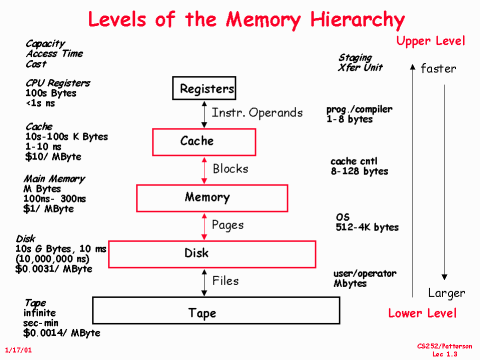
\includegraphics[width=\textwidth]{memory_hierarchy.png} \\
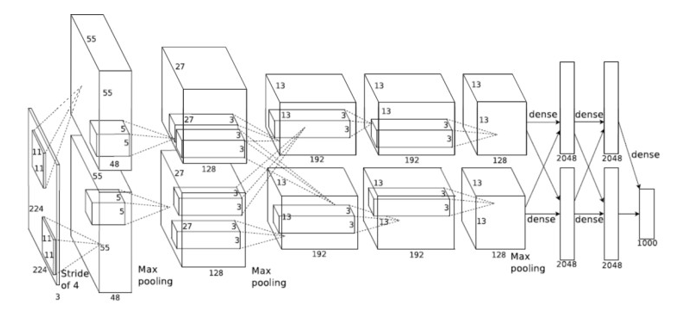
\includegraphics[width=\textwidth]{alexnet_architecture.png} \\
\end{center}
\tiny
GTX 580 GPU has only 3GB of memory
\end{column}
\end{columns}
\end{frame}

\begin{frame}{Probabilistic Programming on deep learning platforms}

\begin{itemize}
\item Edward \url{http://edwardlib.org}
\item PyMC3 \url{https://github.com/pymc-devs/pymc3}
\item pyprob \url{https://github.com/probprog/pyprob}
\item Pyro \url{https://github.com/uber/pyro}
\end{itemize}

\end{frame}

\begin{frame}{GP on deep learning platforms}
GPflow \url{https://github.com/GPflow/GPflow}

GPyTorch \url{https://github.com/cornellius-gp/gpytorch}
\end{frame}



\begin{frame}{MXFusion and GPy2}
\begin{itemize}
\item Beyond GPU acceleration and auto-differentiation
\item Use Gaussian process as a building block.
\item MXFusion: modular probabilistic programming language \\
\url{https://github.com/amzn/MXFusion}
\item GPy2 (a new interface based on MXFusion): 
\begin{itemize}
\item writing new kernel with auto-differentiation
\item scalable inference on GPU
\item Construct hybrid GP, deep GP, recurrent GP by re-using GP module with scalable approximate inference.
\end{itemize}
\end{itemize}
\end{frame}

\begin{frame}{}

Acknowledgement. 

James's blog: \url{https://www.prowler.io/blog/sparse-gps-approximate-the-posterior-not-the-model}
\end{frame}

\bibliographystyle{plainnat}
{\footnotesize
\bibliography{./scalable_gp}
}
%

\end{document}